\documentclass[fleqn]{article}
\oddsidemargin 0.0in
\textwidth 6.0in
\thispagestyle{empty}
\usepackage{import}
\usepackage{amsmath}
\usepackage[backend=bibtex]{biblatex}
\usepackage[utf8]{inputenc}
\usepackage{csquotes}
\usepackage{graphicx}
\usepackage{flexisym}
\usepackage{calligra}
\usepackage{amssymb}
\usepackage{bigints} 
\usepackage[english]{babel}
\usepackage{float}
\usepackage[colorinlistoftodos]{todonotes}
\usepackage{blindtext}
\usepackage{hyperref}

\addbibresource{references.bib}

\hypersetup{
  colorlinks=true,
  linkcolor=blue,
  filecolor=magenta,      
  urlcolor=cyan,
  pdfpagemode=FullScreen
}

\DeclareMathAlphabet{\mathcalligra}{T1}{calligra}{m}{n}
\DeclareFontShape{T1}{calligra}{m}{n}{<->s*[2.2]callig15}{}
\newcommand{\scriptr}{\mathcalligra{r}\,}
\newcommand{\boldscriptr}{\pmb{\mathcalligra{r}}\,}


\setlength{\arrayrulewidth}{0.5mm}
\setlength{\tabcolsep}{18pt}
\renewcommand{\arraystretch}{1.5}


\begin{document}

  \begin{titlepage}

    \newcommand{\HRule}{\rule{\linewidth}{0.5mm}}

    \center

    \begin{center}
      
\includegraphics[height=11cm, width=11cm]{asu.png}
    \end{center}

    \vline

    \HRule \\[0.5cm]
    { \huge \bfseries Particle Collisions In The Universe}\\[0.4cm] 
    \HRule \\[1.0cm]

    \textbf{Behnam Amiri}

    \bigbreak

    \textbf{Prof: Cecilia Lunardini}

    \bigbreak

    \textbf{{\large \today}\\[2cm]}

    \vfill

  \end{titlepage}

  \textbf{What is an elastic collision?}

  \vspace{10px}

  An elastic collision is a collision in which there is no net loss in kinetic energy in the system as a result of 
  the collision. Both momentum and kinetic energy are conserved quantities in elastic collisions. Let's take a look 
  at two-dimensional elastic collision between two billiard balls. Imagine a billiard ball that is going to strike 
  another ball that is stationary.
  \begin{center}
    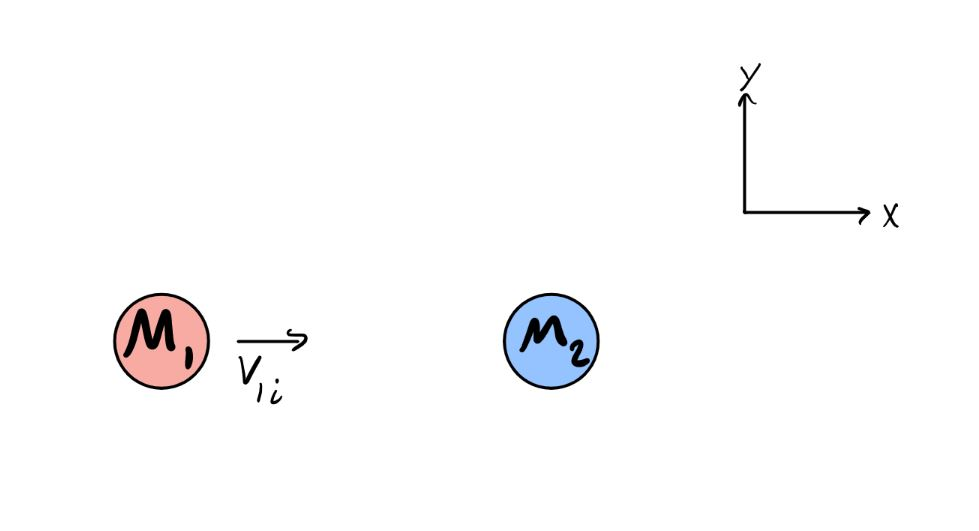
\includegraphics[height=4cm, width=7cm]{1.JPG}
  \end{center}

  Once the first ball hits the second ball, then they both go at different angles.

  \begin{center}
    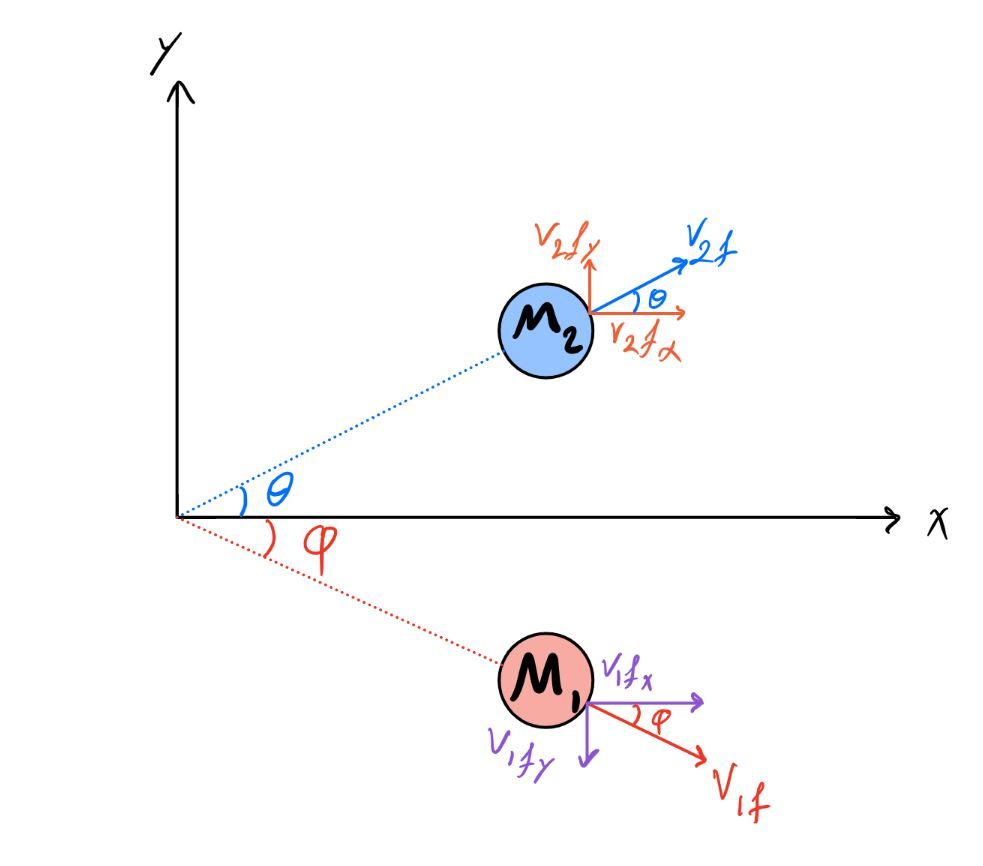
\includegraphics[height=7cm, width=10cm]{2.JPG}
  \end{center}

  Let's see how we can set up conservation of momentum. Since this is a elastic collision that means
  we also have conservation of kinetic energy.

  $
    \\
    \text{Momentum in the x-direction} ~~~ M_1 ~ v_{1i}=M_1 ~ v_{1f} ~ cos(\phi)+M_2 ~ v_{2f} ~ cos(\theta) ~~~~ (1)
    \\
    \\
    \text{Momentum in the y-direction} ~~~ 0=M_2 ~ v_{2f} ~ sin(\theta)-M_1 ~ v_{1f} ~ sin(\phi) ~~~~~~~~~~~ (2)
  $

  \pagebreak

  Conservation of kinetic energy allows us to have:

  $
    \\
    \dfrac{1}{2} M_1 ~ v_{1i}^2=\dfrac{1}{2} M_1 ~ v_{1f}^2+\dfrac{1}{2} M_2 ~ v_{2f}^2 ~~~~~~~~ (3)
  $

  \vspace{10px}

  Assume the two balls have the same mass equals to $M_1=M_2=M$. Then we can rewrite equations $(1), (2),$ and $(3)$.

  $
    \\
    \begin{cases}
      v_{1i}=v_{1f} ~ cos(\phi)+v_{2f} ~ cos(\theta) ~~~~~~~~ (4)
      \\
      \\
      0=v_{2f} ~ sin(\theta)-v_{1f} sin(\phi) ~~~~~~~~ (5)
      \\
      \\
      v_{1i}^2=v_{1f}^2+v_{2f}^2 ~~~~~~~~ (6)
    \end{cases}
    \\
    \\
  $

  Squaring $(4)$ and $(5)$ gives us:

  $
    \\
    \begin{cases}
      v_{1i}^2=v_{1f}^2 ~ cos^2(\phi)+v_{2f}^2 ~ cos^2(\theta)+2 v_{1f} ~ v_{2f} ~ cos(\phi) ~ cos(\theta) ~~~~~~~~ (7)
      \\
      \\
      0=v_{2f}^2 ~ sin^2(\theta)-v_{1f}^2 sin^2(\phi)-2 v_{2f} ~ v_{1f}^2 ~ sin(\theta) ~ sin(\phi) ~~~~~~~~ (8)
    \end{cases}
    \\
    \\
  $

  By adding both equations $(7)$ and $(8)$ we get:

  $
    \\
    v_{1i}^2=v_{1f}^2 \left(sin^2(\phi)+cos^2(\phi)\right)+v_{2f}^2 \left(sin^2(\theta)+cos^2(\theta)\right)
    +2 v_{1f} ~ v_{2f} \left(sin(\theta) ~ cos(\phi)- sin(\phi) ~ sin(\theta)\right)
    \\
    \\
    \\
    \therefore ~~~ v_{1i}^2=v_{1f}^2+v_{2f}^2+2 v_{1f} ~ v_{2f} ~ cos(\theta+\phi) ~~~~~~~~ (9)
    \\
    \\
  $

  Now from equations $(6)$ and $(9)$ we get the following conclusion.

 $
  \\
  v_{1f}^2+v_{2f}^2=v_{1f}^2+v_{2f}^2+2 v_{1f} ~ v_{2f} ~ cos(\theta+\phi) 
  \Longrightarrow 0=2 v_{1f} ~ v_{2f} ~ cos(\theta+\phi)
  \\
  \\
  \\
  \therefore ~~~ \boxed{\theta+\phi=\dfrac{\pi}{2}} ~~~~ \checkmark
  \\
  \\
 $

 For a two dimensional collision where the balls have the same mass, \emph{billiard balls}, they always scatter 
 off at $\dfrac{\pi}{2}$ with each other. In other words, the angle between the two balls after the collision is
 always $\dfrac{\pi}{2}$ when they have the same mass.

\end{document}
